\documentclass[10pt]{article}
\usepackage{geometry}
\geometry{a4paper}




\usepackage{graphicx}
\usepackage{amssymb}
\usepackage{amsmath}
\usepackage{alg}

\usepackage{pgf,tikz}
\usetikzlibrary{arrows,automata}

\usepackage{amsthm}
\theoremstyle{definition}
\newtheorem{thm}{Theorem}
\newtheorem{dfn}[thm]{Definition}
\newtheorem{lem}[thm]{Lemma}
\newtheorem{prop}[thm]{Proposition}
\newtheorem{obs}[thm]{Observation}
\newtheorem{ex}[thm]{Example}
\newtheorem{fact}[thm]{Fact}

\newcommand{\setcomp}[2]{\ensuremath{\{#1\ |\ #2\}}}
\newcommand{\set}[1]{\ensuremath{\{#1\}}}
\newcommand{\tuple}[1]{\ensuremath{\langle#1\rangle}}
\newcommand{\multiset}[1]{\ensuremath{\dot{\{}#1\dot{\}}}}

\newcommand{\kleene}[0]{\ensuremath{^*}}
\newcommand{\familycomp}[2]{\ensuremath{(#1\ |\ #2)}}

\newcommand{\bcup}[1]{\ensuremath{\underset{#1}{\bigcup}\ }}
\newcommand{\bbcup}[2]{\ensuremath{\overset{\!\!\!#1}{\underset{#2}{\bigcup}\ }}}
\newcommand{\bvee}[1]{\ensuremath{\underset{#1}{\bigvee}\ }}
\newcommand{\bbwedge}[2]{\ensuremath{\overset{#1}{\underset{#2}{\bigwedge}\ }}}
\newcommand{\bwedge}[1]{\ensuremath{\underset{#1}{\bigwedge}\ }}
\newcommand{\bsum}[1]{\ensuremath{\underset{#1}{\sum}\ }}

\newcommand{\bisim}{\cong}
\newcommand{\rnarrow}{\rightarrow}

\newcommand{\tripledash}{\ |\!\!\!\equiv}

\newcommand{\commentout}[1]{}

\title{Functional Logic Programming\\with Generalized Circular Coinduction\thanks{I would like to thank Prof.~Dr.~Horst Reichel for his useful input and comments.}}
\author{Ronald de Haan\ \Gamma_{i} = \star(i,\Gamma_{i+1})  \Delta = \star(1,\Delta)  \Lambda = \circ(\Lambda,\Lambda,\ldots)  V = \set{1, 1:y}, \quad E = \set{(1:y,1), (1:y,1:y)}  VL(1) = \emptyset, \quad VL(1:y) = \set{y}  EL(1:y,1) = 1, \quad EL(1:y,1:y) = 2  V' = \set{1,1:y',1:1:y'}, \quad E' = \set{(1:y',1), (1:y',1:1:y'), (1:1:y',1), (1:1:y',1:y')}, VL'(1) = \emptyset, \quad VL'(1:y') = \emptyset, \quad VL'(1:1:y') = \set{y'}  EL'(1:y',1) = 1, \quad EL'(1:1:y',1) = 1  EL'(1:y',1:1:y') = 2, \quad EL'(1:1:y',1:y') = 2  Z = \set{(1,1), (1:y,1:y'), (1:y,1:1:y')}  pos(x,\theta) = \set{\epsilon}  pos(d(t_1,\ldots,t_n),\theta) = \set{\epsilon} \cup \setcomp{1\cdot \overline{m}}{\overline{m} \in pos(t_1)} \cup \cdots \cup \setcomp{n\cdot \overline{m}}{\overline{m} \in pos(t_n)}  \begin{array}{r l l}
(t,\theta)[(t',\theta')]_{\overline{m}} &=& (t[t']_{\overline{m}},(\theta \cup \theta')|_{t[t']_{\overline{m}}}) \\
t[t']_{\epsilon} &=& t' \\
d(t_1,\ldots,t_n)[t']_{i\cdot \overline{m}'} &=& d(t_1,\ldots,t_{i-1},t_{i}[t']_{\overline{m}'},t_{i+1},\ldots,t_n) \\
\end{array}  maxsize(H) - size(H)  (f(g(y,y')),\set{y \mapsto g(y,y'), y' \mapsto h(y')})  \set{ x = f(g(x',x'')), \quad x' = g(x',x''), \quad x'' = h(x'') }  pair(suspend,eq) = suspend  pair(\set{\langle \sigma_1,e_1,M_1\rangle, \ldots, \langle \sigma_n,e_n,M_n \rangle},eq) = \set{\langle \sigma_1,e_1,M_1,eq\rangle,\ldots,\langle \sigma_n,e_n,M_n,eq\rangle}  compose(t,\mathcal{T},\sigma,t',o',M) = \left \{ \begin{array}{l l}

\set{\langle\sigma,t,M\rangle}&\mbox{if }\\
&\mbox{}\\

\\

\{\langle\sigma_1 \circ \sigma,t_1,M_1\rangle, \ldots,&
\mbox{if }\\
\langle \sigma_n \circ \sigma,t_n,M_n\rangle\}&
\mbox{}\\

\end{array} \right .  replace(t,o,suspend) = suspend  replace(t,o,\set{\langle\sigma_1,t_1,M_1,eq_1\rangle,\ldots,\langle\sigma_n,t_n,M_n,eq_n\rangle}) =  \set{\langle\sigma_1,\sigma_1(t)[t_1]_o,M_1,eq_1\rangle,\ldots,\langle\sigma_n,\sigma_1(t)[t_n]_o,M_n,eq_n\rangle}  \begin{array}{r l l l r}

cs(x,t_{tot},o,M)&=&suspend&\mbox{for all variables }&(1)\\
\\
cs(t \doteq t',t_{tot},o,M)&=&\set{\langle \sigma, \top, M, \top \rangle}&\mbox{if  unifies  and }&(2)\\
\\
cs(f(t_1,\ldots,t_n),t_{tot},o,M)&=&pair( cst(f(t_1,\ldots,t_n),\mathcal{T},t_{tot},o,&\mbox{if  is a definitional}&\\
&&M),\top)&\mbox{tree for  and rule (2)}&\\
&&&\mbox{does not apply}&(3.1)\\
&&&\\
&&\cup\\
\\
&&\{ \langle \sigma, g,M,\sigma(t_{tot})[g]_{o} \doteq \sigma(t'_{tot})[g]_{o'}\rangle&\mbox{where }\\
&&|\ \langle t',t'_{tot},o'\rangle \in M, \mbox{ unifies  and}&\\
&&\mbox{,  is a possible guess for } \}&&(3.2)\\
\\
cs(c(t_1,\ldots,t_n),t_{tot},o,M)&=&replace(c(t_1,\ldots,t_n),k,&\mbox{if }\\
&&cs(t_k,t_{tot},o\cdot k,M))&\mbox{, for all }\\
&&&\mbox{and }&\\
&&&\mbox{}&(4)\\
\\
cs(c(t_1,\ldots,t_n),t_{tot},o,M)&=&suspend&\mbox{if }&\\
&&&\mbox{ for all }&(5)\\
\end{array}  cst(t,leaf(l \rightarrow r),t',o',M) = \set{\langle id,\sigma(r), M \cup \set{\langle t,t',o'\rangle}\rangle} \quad \mbox{if  is a substitution with }  \begin{array}{r}
cst(t,branch(\pi,o,\mathcal{T}_1,\\
\ldots,\mathcal{T}_k),t',o',M)\\
\end{array} =
\left \{ \begin{array}{l l}

cst(t,\mathcal{T}_i,t',o',M)&\mbox{if  and}\\
&\mbox{}\\
\\
\emptyset&\mbox{if  and}\\
&\mbox{, }\\
\\
\bigcup^k_{i=1} compose(\sigma_i(t),\mathcal{T}_i,\sigma_i,t',o',M)&\mbox{if  and}\\
&\mbox{}\\
\\
replace(t,o,cs(t|_o,t',o'\cdot o,M))&\mbox{if }\\
\end{array} \right .  \top \wedge X \rightarrow X  X \wedge \top \rightarrow X  (\top \Rightarrow X) \rightarrow X  D \vee \langle \sigma, e, M \rangle \vee D' \rnarrow D \vee \langle \sigma_1 \circ \sigma, eq_1 \Rightarrow e_1, M_1 \rangle \vee \ldots \vee \langle \sigma_n \circ \sigma, eq_n \Rightarrow e_n, M_n \rangle \vee D'  \mbox{if  is unsolved and } } (1);
\end{tikzpicture}
\hspace{20pt}
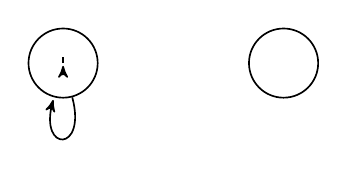
\begin{tikzpicture}[->,>=stealth',shorten >=1pt,auto,node distance=2.8cm,semithick]
  \tikzstyle{every state}=[]
  \node[state] (2) {};
  \node[state] (3) [right of=2] {};
  \path (2) edge [loop below] node {} (3);
  \path (2) edge [bend left] node {} (2);
\end{tikzpicture}
\end{center}

\begin{figure}[h]
\begin{center}
\textbf{Reduction rules:}\\
\begin{verbatim}
-- kripke structures
state "m1" = 1
trans "m1" 1 = 1
val "m1" 1 = 'p'

state "m2" = 2
state "m2" = 3
trans "m2" 2 = 2
trans "m2" 2 = 3
trans "m2" 3 = 2
trans "m2" 3 = 3
val "m2" 2 = 'p'
val "m2" 3 = 'p'

-- mechanism
bisim m1 w1 m2 w2 =
  let next1 = findall (trans m1 w1)
  and next2 = findall (trans m2 w2) in
    sameSet (findall (val m1 w1)) (findall (val m2 w2)) &&
    forall (\v1 -> (exists (\v2 -> bisim m1 v1 m2 v2) next2) next1) &&
    forall (\v2 -> (exists (\v1 -> bisim m1 v1 m2 v2) next1) next2)

and [] = True
and (x:xs) = x && (and xs)

forall f xs = and (map f xs)
exists f xs = not (and (map (\x -> not (f x)) xs))

sameSet xs ys = (subSet xs ys) && (subSet ys xs)
subSet [] _ = True
subSet (x:xs) ys = (elem x ys) && subSet xs ys
\end{verbatim}

\vspace{5pt}\textbf{Assumption possibilities:}\\
\begin{tabular}{l l l}
\verb|and _| &  & \verb|{True}| \\
\verb|bisim _ _ _ _| &  & \verb|{True}| \\
\end{tabular}
\end{center}
\caption{Example program .}
\label{fig:ex3}
\end{figure}

We can make the following derivations by using program . These example derivations illustrate that the direct encoding of the bisimulation conditions directly lead to a decision procedure.

\vspace{10pt}\begin{tabular}{l l l l}
\textbf{term}&&\textbf{value}&\textbf{substitution}\\
\verb|bisim "m1" 1 "m2" 2| && \verb|True|\\
\verb|bisim "m1" 1 "m2" x| && \verb|True| & \verb|{x -> 3}|\\
\end{tabular}\vspace{10pt}

Similarly to the example of B\"uchi automata given above, it is possible to encode bisimulation of Kripke structures in regular Curry, but not nearly as directly and straightforwardly as in our approach.

\subsection{Manipulation of infinite lists}

In the program  in Figure~\ref{fig:ex4}, we consider manipulation of infinite lists. This example shows that we can directly use the definition of several list manipulation operators from the finite case also in the infinite case (with regular terms), with the intended interpretation.

\begin{figure}[h]
\begin{center}
\textbf{Reduction rules:}\\
\begin{verbatim}
zip [] ys = ys
zip (x:xs) (y:ys) = x:y:(zip xs ys)

odd [] = []
odd (x:xs) = x:(even xs)

even [] = []
even (x:xs) = odd xs

ones = 1:ones
twos = 2:twos

nat n = n:(nat (n+1))
\end{verbatim}

\vspace{5pt}\textbf{Assumption possibilities:}\\
\begin{tabular}{l l l}
\verb|zip _ _| &  & \verb|{_}| \\
\verb|odd _| &  & \verb|{_}| \\
\end{tabular}
\end{center}
\caption{Example program .}
\label{fig:ex4}
\end{figure}

We can make the following derivations by using program . These examples show that the operations \verb|zip|, \verb|even| and \verb|odd| can be naturally used for infinite lists as well as finite lists. An equally natural encoding of such operations on infinite lists in regular Curry is not possible.

\vspace{10pt}\begin{tabular}{l l l l}
\textbf{term}&&\textbf{value}&\textbf{substitution}\\
\verb|zip ones twos| && \verb|1:2:y {y -> 1:2:y}|\\
\verb|zip ones ones| && \verb|1:1:y {y -> 1:1:y}|\\
\verb|odd (zip ones x)| && \verb|1:y {y -> 1:y}|&(see below)\\
\verb|even (zip x twos)| && \verb|2:y {y -> 2:y}|&(see below)\\
\verb|odd ones| && \verb|1:y {y -> 1:y}|\\
\verb|even ones| && \verb|1:y {y -> 1:y}|\\
\end{tabular}\vspace{10pt}

No derivation for \verb|odd (zip ones x)| and \verb|even (zip x twos)| leading to the mentioned values has an empty substitution. Each derivation results in a substitution mapping \verb|x| to an infinite list (representable by a cyclic term). Furthermore, for every substitution mapping \verb|x| to any cyclic term representing an infinite list (containing only fresh variables), there is a derivation leading to the mentioned values with this substitution.

Note that the term \verb|nat n|, for any integer \verb|n|, is infinite and non-regular. Our computational strategy is not suited to reason about such terms. This example illustrates this. We have that evaluating the following terms results in a diverging derivation. Similar effects occur when such non-regular infinite terms are used in the previous examples.

\vspace{10pt}\begin{tabular}{l l l}
\textbf{term}\\
\verb|odd (zip ones (nat 1))| && \ldots\\
\verb|even (zip (nat 1) twos)| && \ldots\\
\end{tabular}

\section{Declarative semantics}\label{sec:declsem}

Naturally, when modifying the operational semantics to interpret programs coinductively, we would like to change the denotational, or declarative, semantics accordingly. In this section, we suggest a possibility for suitable denotational semantics. Also, by means of several examples we illustrate how this suggested semantics differs from the inductive case. Furthermore, these examples serve to illustrate the suitability of the suggested semantics for the coinductive case.

For inductively interpreted functional logic programs, initial algebra denotational semantics is well-suited. Dually, for coinductively interpreted functional logic programs, we suggest a final coalgebra denotational semantics. For a general background on algebrae and coalgebrae, see for instance \cite{Jacobs:1997p238}. Consider the following (partial) signature specifying a particular type \textit{List}:

Intuitively, in the inductive case, terms (of type ) correspond to finite lists of natural numbers. In the coinductive case, intuitively, cyclic terms (of type ) correspond to finite or infinite lists of natural numbers.

A suitable denotational semantics for terms of type  is the initial -algebra on the category of sets , where the corresponding functor  is derived directly from the signature. Call this initial algebra .\footnote{There are more such initial -algebrae on , but they are all isomorphic.} Terms correspond to elements of . In fact, the set of finite lists on  is a suitable initial algebra. Now, functions from terms to natural numbers get the denotation of an -algebra on , functions from terms to terms get the denotation of an -algebra on . For instance, the (Curry encoding of the) function  returning the length of a list would denote the algebra , given by:


By initiality of , there is exactly one morphism from  to this algebra on , which coincides with the function returning the length of lists in . Also, for instance, pairs of terms of type  are assigned the denotation of elements in the algebra . In an analogous fashion, denotational semantics in algebraic terms can be assigned to the complete program.

The suggested final coalgebra semantics for cyclic terms of type  are completely dual to the initial algebra semantics for the inductive case. In this semantics, cyclic terms denote elements of the final -coalgebra on , where the corresponding functor  is derived directly from the signature. Call this final coalgebra .\footnote{There are more such final -coalgebrae on , but they are all isomorphic.} Cyclic terms correspond to elements of . In fact, the set of all finite and infinite lists on  is a suitable final coalgebra. Assigning denotations to functions works dually to the inductive case. Functions from natural numbers to cyclic terms are -coalgebrae on , and functions from cyclic terms to cyclic terms are -coalgebae on . For instance, the function \verb|repeat| from natural numbers to cyclic terms given by \verb|repeat n = (n::(repeat n))| would denote the coalgebra , given by:


By finality of , there is exactly one morphism from this coalgebra on  to , which coincides with the function mapping any natural number to the infinite list containing only this number. Also, for instance, pairs of cyclic terms are assigned the denotation of elements in the coalgebra . Again, analogously, the whole program can be assigned denotational semantics in coalgebraic terms.

The above exposition is a gross oversimplification, of course. Things get more intricate, for instance, when a program is interpreted partially inductively and partially coinductively. Further research is needed on the topic of denotational semantics. We merely suggest a direction for research in this area.

\section{Conclusions}\label{sec:conclusions}
We showed how functional logic programming can be adapted to interpret programs coinductively as well as inductively. We singled out a particular class of (possibly infinite) objects interesting for this kind of reasoning, namely regular terms, and showed how the usual data structures can be modified to capture these objects. We showed how the operational semantics of the functional logic programming language Curry can be altered to allow for coinductive reasoning, and suggested how a suitable declarative semantics can be obtained. Furthermore, we illustrated the working and usefulness of our methods with several examples.

Working out a declarative semantics in full detail, and relating this semantics to the operational semantics, would be a topic of further research. Another direction for further research would be to investigate whether and how the computational mechanisms used in this paper could be optimized.

\bibliographystyle{ieeetr}
\bibliography{bibliography}

\listoftodos

\pagebreak
\appendix
\section{Example derivations}\label{sec:examplederivations}
In Figure~\ref{fig:examplederivations}, we include several derivations for the example programs given in Section~\ref{sec:examples}. For each derivation, we indicate certain (meaningful) steps in the derivation, together with the cases of the function  used to get from the previous step to this step (indicated in the column titled \textbf{case of }), and the (partial) resulting substitution calculated in the derivation from the previous step to this step (indicated in the column titled ).

\begin{figure}[h!]
\begin{footnotesize}
\begin{center}

\begin{tabular}{l l l l}
&\textbf{term}&\textbf{case(s) of }&\\
&\verb|forall isOdd ones|&\\
&\verb|and (map isOdd ones)|&(3.1)\\
&\verb|and ((isOdd 1):(map isOdd ones))|&(3.1)\\
&\verb|and (True:(map isOdd ones))|&(3.1)\\
&\verb|True && (and (map isOdd ones))|&(3.1)\\
&\verb|and (map isOdd ones)|&(3.1)\\
&\verb|True|&(3.2), (2), (3.1)\\
\\ \\
&\textbf{term}&\textbf{case(s) of }&\\
&\verb|append ones [2,3]|&\\
&\verb|1:(append ones [2,3])|&(3.1)\\
&\verb|(x1 == 1:x1) => x1|&(3.2)\\
&\verb|True => y1 {y1 -> 1:y1}|&(2)&\verb|{x1 -> y1 {y1 -> 1:y1}}|\\
&\verb|y1 {y1 -> 1:y1}|&(3.1)\\
\\ \\
&\textbf{term}&\textbf{case(s) of }&\\
&\verb|accept x|&\\
&\verb|inf (==final) (path initial x)|&(3.1)\\
&\verb|inf' (==final) False (loop (path initial x))|&(3.1)\\
&\verb|inf' (==final) False (loop (1:(path 2 x2)))|&(3.1)&\verb|{x -> (a:x2)}|\\
&\verb|inf' (==final) False (loop (path 2 x2))|&(3.1)&\\
&\verb|inf' (==final) False (loop (2:(path 2 x3)))|&(3.1)&\verb|{x2 -> (b:x3)}|\\
&\verb|inf' (==final) False (loop (path 2 x3))|&(3.1)&\\
&\verb|inf' (==final) False (path 2 y1) {y1 -> b:y1}|&(3.2), (2), (3.1)&\verb|{x3 -> y1 {y1 -> b:y1}}|\\
&\verb+inf' (==final) ((2==final) || False) (path 2 y1)+&(3.1)&\\
&\verb|inf' (==final) True (path 2 y1) {y1 -> b:y1}|&(3.1)&\\
&\verb|inf' (==final) True (path 2 y1) {y1 -> b:y1}|&(3.1)&\\
&\verb|True|&(3.2), (2), (3.1)&\\
\\ \\
&\textbf{term}&\textbf{case(s) of }&\\
&\verb|odd (zip ones x)|&\\
&\verb|odd (1:x1:(zip ones xs1))|&(3.1)&\verb|{x -> (x1:xs1)}|\\
&\verb|1:(odd (zip ones xs1))|&(3.1)&\\
&\verb|(x2 == 1:x2) => x2|&(3.2)&\verb|{x -> y1, xs1 -> y1|\\
&&&\verb|         {y1 -> x1:y1}}|\\
&\verb|True => y2 {y2 -> 1:y2}|&(2)&\verb|{x2 -> y2 {y2 -> 1:y2}}|\\
&\verb|y2 {y2 -> 1:y2}|&(3.1)&\\
\end{tabular}

\end{center}
\end{footnotesize}
\caption{Example derivations.}
\label{fig:examplederivations}
\end{figure}

\end{document}